\chapter{Présentation et principes de base}
\label{chap:presentation}


{\LaTeX} est certainement

{\TeX}, {\LaTeX}, {\XeLaTeX}, {\LuaTeX}

Un peu de phonétique avant d'aller plus loin. La dernière lettre de
tous les acronymes ci-dessus étant non pas un X, mais plutôt la lettre
grecque khi majuscule (visuellement identique), la terminaison se
prononce «tek». Voilà qui devrait permettre de distinguer
immédiatement le système de mise en page du matériau élastique.

de {\TeX}, {\LaTeX} et consorts

\section{Ce que c'est}
\label{sec:presentation:c-est}

À la base de {\LaTeX} et de ses dérivés, il y a toujours le système
{\TeX} développé par Donald Knuth à partir de la fin des années 1970
alors qu'il travaillait à la rédaction de son {\oe}uvre phare
\emph{The Art of Computer Programming}. Comme il n'était pas satisfait
de la qualité typographique des systèmes de mise en page alors
disponibles, il a tout naturellement décidé d'en créer un à la hauteur
de ses exigences!

\begin{itemize}
\item {\TeX} est un système de mise en page (\emph{typesetting}) ou de
  préparation de documents.
\item {\LaTeX} est un ensemble de macro-commandes développé par Leslie
  Lamport en 1983 pour faciliter l'utilisation de {\TeX}. Le terme
  {\LaTeX} en est venu, chez les utilisateurs, à nommer l'ensemble du
  système.
\item {\TeX} et {\LaTeX} sont des langages de balisage (\emph{Markup
    Languages}) qui indiquent la mise en forme du texte à l'intérieur
  de celui-ci.
\item {\TeX} met l'accent sur la production de documents de grande
  qualité à la typographie soignée, surtout pour les mathématiques.
\end{itemize}

\begin{exemple}
  Les traitements de texte sont d'abord et avant tout conçus pour
  reproduire à l'identique ce que l'utilisateur produit à l'écran
  (d'où l'appellation \emph{What You See is What You Get}, WYSIWYG).
  Les systèmes de mise en page, eux, visent plutôt à produire une mise
  en page et une typographie de grande qualité pour un texte donné.

  Voici deux exemples de typographie soignée. D'abord, l'utilisation
  de \emph{ligatures} (jonctions) entre certaines lettres. À gauche,
  ce que produisent les traitements de texte, qui ne voient qu'une
  série de lettres individuelles. À droite, le résultat avec {\LaTeX},
  qui peut analyser le texte et identifier les ligatures.
  \begin{demo}
    \centering
    \begin{minipage}{0.3\linewidth}
      \rmfamily f\/f \quad f\/i \quad f\/l \quad f\/f\/i \quad
      f\/f\/l
    \end{minipage}
    \qquad
    \begin{minipage}{0.3\linewidth}
      \rmfamily ff \quad fi \quad fl \quad ffi \quad ffl
    \end{minipage}
  \end{demo}

  Ensuite, l'espacement entre les lettres. {\LaTeX} l'ajustera selon
  le contexte. Comparer la disposition pour du texte normal, à gauche,
  à celle pour des mathématiques, à droite.
  \begin{demo}
    \centering
    \begin{minipage}{0.3\linewidth}
      \rmfamily xy \quad \emph{xy}
    \end{minipage}
    \qquad
    \begin{minipage}{0.3\linewidth}
      $xy$
    \end{minipage}
  \end{demo}
  \qed
\end{exemple}


\section{Ce que ce n'est pas}
\label{sec:presentation:n-est-pas}

\begin{itemize}
\item Un traitement de texte --- {\LaTeX} impose un mode de travail
  qui permet de séparer \emph{structure} et \emph{apparence} du texte.
\item WYSIWYG --- un système de mise en page est davantage qualité de
  \emph{What You See is What You Mean}.
\item Incompatible --- le code source {\LaTeX} peut être lu et le
  document reproduit à l'identique sur tous les types de systèmes
  informatiques.
\item Instable --- le moteur {\TeX} est considéré exempt de bogues.
\item Imprévisible --- {\LaTeX} fait uniquement et exactement ce qu'on
  lui demande, sans prétendre pouvoir deviner ce que nous voulons
  faire ou, pire, le savoir mieux que nous.
\end{itemize}


\section{Processus de création d'un document}

Le processus de création d'un document {\LaTeX} compte trois phases:
la rédaction, la compilation (ou composition par le système) et la
visualisation du résultat. On peut le représenter schématiquement
ainsi:
\begin{center}
  \begin{minipage}[t]{0.25\linewidth}
    \centering
    {\Huge\faFileTextO} \\ \medskip
    rédaction du texte et balisage avec un \emph{éditeur de texte}
  \end{minipage}
  \quad{\Large\faArrowRight}\quad
  \begin{minipage}[t]{0.25\linewidth}
    \centering
    {\Huge\faCogs} \\ \medskip
    compilation avec un \emph{moteur} {\TeX} depuis la ligne de commande
  \end{minipage}
  \quad{\Large\faArrowRight}\quad
  \begin{minipage}[t]{0.25\linewidth}
    \centering
    {\Huge\faFilePdfO} \\ \medskip
    visualisation avec une visionneuse externe (Aperçu,
    SumatraPDF, etc.)
  \end{minipage}
\end{center}

Les logiciels de rédaction intégrés facilitent grandement les deux
premières étapes --- certains intègrent même une visionneuse PDF pour
englober le processus au complet. Il existe plusieurs de ces
logiciels. Mentionnons, par exemple:
\begin{itemize}
\item \link{http://www.xm1math.net/texmaker/index_fr.html}{Texmaker}
  (multiplateforme);
\item \link{http://www.tug.org/texworks/}{TeXworks} (multiplateforme);
\item \link{http://www.texshop.org/}{TeXShop} (OS~X seulement);
\item \link{http://www.winedt.com}{WinEdt} (Windows seulement);
\item \link{http://kile.sourceforge.net}{Kile} (Linux);
\item à peu près tous les bons éditeurs de texte pour programmeur.
\end{itemize}

\section{Quelques choses simples à réaliser avec {\LaTeX} }

Quiconque a travaillé un tant soit peu les logiciels de traitement de
texte reconnaîtra ci-dessous des éléments de mise en page qui ne sont
pas toujours faciles à réaliser. C'est tout le contraire avec
{\LaTeX}: quand ce n'est pas le comportement par défaut, il suffit en
général d'insérer une commande dans le code source pour obtenir le
résultat souhaité.

\begin{itemize}
\item Page titre standard avec le titre du document, le nom de
  l'auteur et la date (une commande).
\item Table des matières (une commande).
\item Numérotation des pages (automatique).
\item Disposition sur la page des figures et tableaux, numérotation et
  renvois.
\item Numérotation des équations mathématiques et renvois (automatique).
\item Citations et composition de la bibliographie.
\item Coupure de mots (automatique).
\item Document recto-verso avec marges distinctes pour le recto et le
  verso (une commande).
\end{itemize}


\section{Outils de production}

Le \autoref{tab:presentation:moteurs} dresse la liste des divers
\emph{moteurs} {\TeX} et formats (ensembles de macro commandes)
couramment utilisés aujourd'hui.

\begin{table}
  \centering
  \begin{tabular}{llc}
    \toprule
    Moteur & Format & Fichier de sortie \\
    \midrule
    \code{tex} & \emph{plain} \TeX & DVI \\
    \code{tex} (\code{latex}) & \LaTeX & DVI \\
    \code{pdftex} (\code{pdflatex}) & pdf\LaTeX & PDF \\
    \code{xetex} (\code{xelatex}) & \XeLaTeX & PDF \\
    \code{luatex} (\code{lualatex}) & \LuaLaTeX & PDF \\
    \bottomrule
  \end{tabular}
  \caption{Moteurs et formats les plus courants}
  \label{tab:presentation:moteurs}
\end{table}

\begin{itemize}
\item Les formats les plus usuels sont pdf{\LaTeX} et {\XeLaTeX}. La
  classe \class{ulthese} est compatible avec les deux.
\item Le moteur \code{pdftex} est le moteur par défaut des
  distributions {\LaTeX} modernes. Comme son nom l'indique, ce moteur
  produit directement un fichier de sortie en format PDF. C'est la
  principale différence par rapport au moteur \code{tex}.
\item Le moteur \code{xetex} peut utiliser directement les polices de
  caractères du système d'exploitation. On traite de l'utilisation des
  polices de caractères plus en détail à la \autoref{trucs:polices}.
\item Le format de fichier de sortie DVI, qui est antérieur aux
  formats PostScript et PDF, permet de décrire la disposition d'un
  document exactement telle qu'elle devrait apparaître à l'écran ou à
  l'impression. C'est un format aujourd'hui plus ou moins tombé en
  désuétude depuis la standardisation autour du format PDF.
\end{itemize}

Le système {\LaTeX} est formé d'un grand nombre de composantes réunies
sont forme d'une \emph{distribution}. La plus populaire distribution
aujourd'hui est %
\link{https://www.tug.org/texlive}{{\TeX}~Live}. %
Elle est administrée par le {\TeX} Users Group. C'est la distribution que
recommandent la Bibliothèque et la Faculté des études supérieures de
l'Université Laval.

\begin{itemize}
\item Sous OS~X, on installera plutôt la distribution %
  \link{https://www.tug.org/mactex/}{Mac{\TeX}}, %
  qui est étroitement dérivée de {\TeX}~Live.
\item Sous Windows, la distribution %
  \link{http://www.miktex.org}{MiK\TeX} %
  demeure aussi très populaire.
\item La philosophie de {\TeX}~Live: tout installer. Cette façon de
  faire est aujourd'hui réalisable puisque l'espace disque est
  disponible à profusion dans les ordinateurs. C'est également la plus
  simple puisque à peu près tout ce que vous êtes susceptible
  d'utiliser dans un système {\TeX} est déjà installé.
\end{itemize}


\begin{information}
  Quelques faits amusants au sujet de {\TeX}.
  \begin{itemize}
  \item {\TeX} est aujourd'hui considéré essentiellement exempt de
    bogue.
  \item Donald Knuth vous offre une récompense (symbolique) si vous en
    trouvez un!
  \item Le numéro de version de {\TeX} converge vers $\pi$:
\begin{lstlisting}
$ tex --version
TeX `\textbf{3.14159265}' (TeX Live 2015)
kpathsea version 6.2.1
Copyright 2015 D.E. Knuth.
[...]
\end{lstlisting}
  \end{itemize}
  Pour en savoir plus:
  \begin{itemize}
  \item \link{https://www.tug.org/whatis.html}{Histoire de \TeX} sur le
    site du {\TeX} Users Group (en anglais);
  \item {\TeX} sur Wikipedia
    (\link{http://fr.wikipedia.org/wiki/TeX}{version française};
    \link{http://en.wikipedia.org/wiki/TeX}{version anglaise}, plus
    complète).
  \end{itemize}
\end{information}

\section{Rédaction}

On se concentre sur le contenu et la \emph{structure} du document,
pas sur son \emph{apparence}.

\begin{itemize}
\item Par exemple: \bigskip
  \begin{tabbing}
    \verb=\textbf{titre}= \qquad\= \faArrowRight \qquad\= \verb|\section{titre}| \\[6pt]
    \verb|\textit{texte}| \> \faArrowRight \> \verb|\emph{texte}|
  \end{tabbing}
  \bigskip
\item L'apparence du texte est prise en charge par {\LaTeX}. Les
  gabarits étant l'{\oe}uvre de spécialistes, il est généralement
  préférable de ne pas les modifier.
\item Dans {\LaTeX}, on sépare:
  \begin{itemize}
  \item les mots par une ou plusieurs \emph{espaces} (la mise en page
    sera la même peu importe le nombre d'espaces dans le code source);
  \item les paragraphes par une ou plusieurs lignes blanches
    (celles-ci n'apparaîtront pas nécessairement dans le texte final).
  \end{itemize}
\item On aura recours à des \emph{commandes} pour indiquer la
  structure du texte dans le code source.
\end{itemize}


\section{Structure d'un document}

Un fichier source {\LaTeX} est toujours composé de deux parties.

\begin{enumerate}
\item Le \emph{préambule}:
  \begin{itemize}
  \item suite de commandes spécifiant la mise en forme globale
    du document (format du papier, marges, entête et pied de page,
    etc.);
  \item contient au minimum la commande \cmd{\documentclass}.
  \end{itemize}
\item Le \emph{corps} du document:
  \begin{itemize}
  \item débute par \verb=\begin{document}=;
    \item contient le texte du document;
    \item contient presque toujours des commandes à effet
      \emph{local};
    \item se termine par \verb=\end{document}=.
  \end{itemize}
\end{enumerate}


\section{Commandes}

\begin{itemize}
\item Le nom des commandes débute toujours par {\bs}.
\item Le nom d'une commande se termine par tout caractère qui n'est
  pas une lettre (y compris l'espace!). Cette règle joue parfois de
  vilains tours; voir l'\autoref{ex:base:commandes}.
\item Les commandes peuvent avoir:
  \begin{itemize}
  \item aucun argument;
  \item un ou plusieurs arguments obligatoires placés entre accolades
    \verb={ }=;
  \item un ou plusieurs arguments optionnels placés entre crochets
    \verb=[ ]=;
  \end{itemize}
\item Les formes générales des commandes sont:
\begin{lstlisting}
\`\meta{nomcommande}\oarg{arg\_optionnel}\marg{arg\_obligatoire}'
\`\meta{nomcommande}'*`\oarg{arg\_optionnel}\marg{arg\_obligatoire}'
\end{lstlisting}
  La forme étoilée d'une commande réalise généralement une action
  légèrement différente de la version sans étoile. Par exemple, la
  commande \cmd{\section} crée une nouvelle section numérotée, alors
  que \cmd{\section*} n'insère aucune numérotation.
\item La portée d'une commande est limitée à la zone entre accolades
  \verb={ }=, le cas échéant.
\end{itemize}


\section{Environnements}

\begin{itemize}
\item Les environnements sont délimités par des constructions du type
\begin{lstlisting}
\begin{`\meta{environnement}'}
   ...
\end{`\meta{environnement}'}
\end{lstlisting}
\item Le contenu d'un environnement est traité différemment du reste
  du texte. Par exemple, le texte à l'intérieur d'un environnement
  \Ie{center} est centré sur la page.
\item Les changements induits par un environnement s'appliquent
  uniquement à l'intérieur de celui-ci.
\end{itemize}


\section{Caractères spéciaux}

\begin{itemize}
\item Certains caractères sont réservés par {\TeX}:
  \begin{demo}
    \verb=# $ & ~ _ ^ % { }=
  \end{demo}
\item Pour les utiliser dans le texte, il faut les précéder par le caractère {\bs}:
  \begin{demo}
    \begin{minipage}{0.3\linewidth}
      \begin{texample}
\begin{lstlisting}
\#
\end{lstlisting}
        \producing\#
      \end{texample}
    \end{minipage}
    \hfill
    \begin{minipage}{0.3\linewidth}
      \begin{texample}
\begin{lstlisting}
\$
\end{lstlisting}
        \producing\$
      \end{texample}
    \end{minipage}
    \hfill
    \begin{minipage}{0.3\linewidth}
      \begin{texample}
\begin{lstlisting}
\%
\end{lstlisting}
        \producing\%
      \end{texample}
    \end{minipage}
    \\
    \begin{minipage}{0.3\linewidth}
      \begin{texample}
\begin{lstlisting}
\_
\end{lstlisting}
        \producing\_
      \end{texample}
    \end{minipage}
    \hfill
    \begin{minipage}{0.3\linewidth}
      \begin{texample}
\begin{lstlisting}
\{
\end{lstlisting}
        \producing\}
      \end{texample}
    \end{minipage}
    \hfill
    \begin{minipage}{0.3\linewidth}
      \begin{texample}
\begin{lstlisting}
\}
\end{lstlisting}
        \producing\}
      \end{texample}
    \end{minipage}
  \end{demo}
%
\item Les guillemets nécessitent un traitement particulier:
  \begin{demo}
    \begin{texample}
\begin{lstlisting}[escapeinside={}]
``guillemets anglais''
\end{lstlisting}
      \producing
      ``guillemets anglais''
    \end{texample} \\
    \begin{texample}
\begin{lstlisting}
«guillemets français»
\end{lstlisting}
      \producing
      «guillemets français»
    \end{texample}
  \end{demo}
%
\item {\LaTeX} permet de créer facilement le tiret, le tiret
  demi-cadratin et le tiret cadratin:
  \begin{demo}
    \begin{minipage}{0.3\linewidth}
      \begin{texample}
\begin{lstlisting}
-
\end{lstlisting}
        \producing
        -
      \end{texample}
    \end{minipage}
    \hfill
    \begin{minipage}{0.3\linewidth}
      \begin{texample}
\begin{lstlisting}
--
\end{lstlisting}
        \producing
        --
      \end{texample}
    \end{minipage}
    \hfill
    \begin{minipage}{0.3\linewidth}
      \begin{texample}
\begin{lstlisting}
---
\end{lstlisting}
        \producing
        ---
      \end{texample}
    \end{minipage}
  \end{demo}
\end{itemize}


\section{Classes et paquetages}

La première commande du préambule est normalement la déclaration de la
\emph{classe} du document.
\begin{itemize}
\item La forme de la déclaration est la suivante:
\begin{lstlisting}
\documentclass`\oarg{options}\marg{classe}'
\end{lstlisting}
\item Les classes standards de {\LaTeX} sont \class{article},
  \class{report}, \class{book}, \class{letter} et \class{slides}.
\item La classe pour les thèses et mémoires de l'Université Laval se
  nomme \class{ulthese}. Celle-ci se base sur la classe \class{memoir}
  et, par conséquent, hérite de toutes ses (nombreuses)
  fonctionnalités.
\item Les options disponibles varient d'une classe à l'autre. Les
  options les plus courantes sont les suivantes:
  \begin{description}
  \item[\code{10pt}, \textbf{\code{11pt}}, \code{12pt}] taille de la
    police du document;
  \item[\textbf{\code{oneside}}, \code{twoside}] document recto
    seulement ou recto-verso;
  \item[\textbf{\code{openright}}, \code{openany}] ouverture des
    chapitres toujours à droite ou immédiatement après la dernière
    page du chapitre précédent;
  \item[\code{article}] mise en page d'un article plutôt que celle
    d'un livre (classe \class{memoir}).
  \end{description}
  Les options en caractères gras sont actives par défaut avec la
  classe \class{ulthese}.
\end{itemize}

Les \emph{paquetages} permettent de modifier des commandes ou
d'ajouter des fonctionnalités à {\LaTeX}.
\begin{itemize}
\item On charge les paquetages dans le préambule avec des commandes de
  la forme
\begin{lstlisting}
\usepackage`\marg{paquetage}'
\usepackage`\oarg{options}\marg{paquetage}'
\usepackage`\marg{paquetage1,paquetage2,...}'
\end{lstlisting}
\item Les incontournables:
  \begin{description}
    %% \hfill = PMLA (Poor Man's Left Align) !
  \item[babel*\hfill] typographie multilingue
  \item[inputenc*\hfill] composition en français (\LaTeX)
  \item[fontspec*\hfill] contrôle des polices (\XeLaTeX)
  \item[amsmath\hfill] extensions mathématiques
  \item[booktabs*\hfill] amélioration des tableaux
  \item[hyperref*\hfill] hyperliens dans PDF
  \end{description}
  {\footnotesize * = chargé par défaut dans \class{ulthese}}
\end{itemize}

\section{{\LaTeX} en français}

  \begin{tabularx}{1.0\linewidth}{Xl}
    \toprule
    \textbf{Enjeu} & \textbf{Solution} \\
    \midrule
    \addlinespace[6pt]
    traduction des mots-clés prédéfinis & \pkg{babel} \\
    \addlinespace[6pt]
    coupure de mots & \pkg{babel} \\
    \addlinespace[6pt]
    typographie française & \pkg{babel} \\
    \addlinespace[6pt]
    lettres accentuées dans source & \pkg{inputenc} (\LaTeX) \\
                                   & source en UTF-8 (\XeLaTeX) \\
    \addlinespace[6pt]
    virgule comme séparateur décimal & \pkg{icomma}, \pkg{ncccomma} \\
    \addlinespace[6pt]
    espace comme séparateur des milliers & \pkg{numprint}
  \end{tabularx}



%%%
%%% Exercices
%%%

\section{Exercices}
\label{sec:presentation:exercices}

\begin{exercice}[nosol]
  Démarrer le logiciel Texmaker (ou tout autre éditeur ou logiciel
  intégré de rédaction de votre choix), puis ouvrir et compiler le
  fichier \fichier{exercice\_minimal.tex}.
\end{exercice}

\begin{exercice}[nosol]
  Utiliser le fichier \fichier{exercice\_minimal.tex}.
  \begin{enumerate}
  \item Compiler le document avec la classe \class{article}, puis avec
    la classe \class{book}. Observer le résultat.
  \item Ajouter du texte en français (avec accents) et observer le
    résultat.
  \end{enumerate}
\end{exercice}

\begin{exercice}[nosol]
  Question de voir ce que {\LaTeX} peut faire, compiler le document
  élaboré \fichier{exercice\_demo.tex} de la manière suivante:
  \begin{enumerate}[i)]
  \item une fois avec {\LaTeX};
  \item une fois avec {\BibTeX};
  \item deux à trois autres fois avec {\LaTeX}.
  \end{enumerate}
\end{exercice}

\begin{exercice}[nosol]
  \label{ex:base:commandes}
  Modifier le fichier \fichier{exercice\_commandes.tex} afin
  de produire le texte ci-dessous.
  \begin{center}
    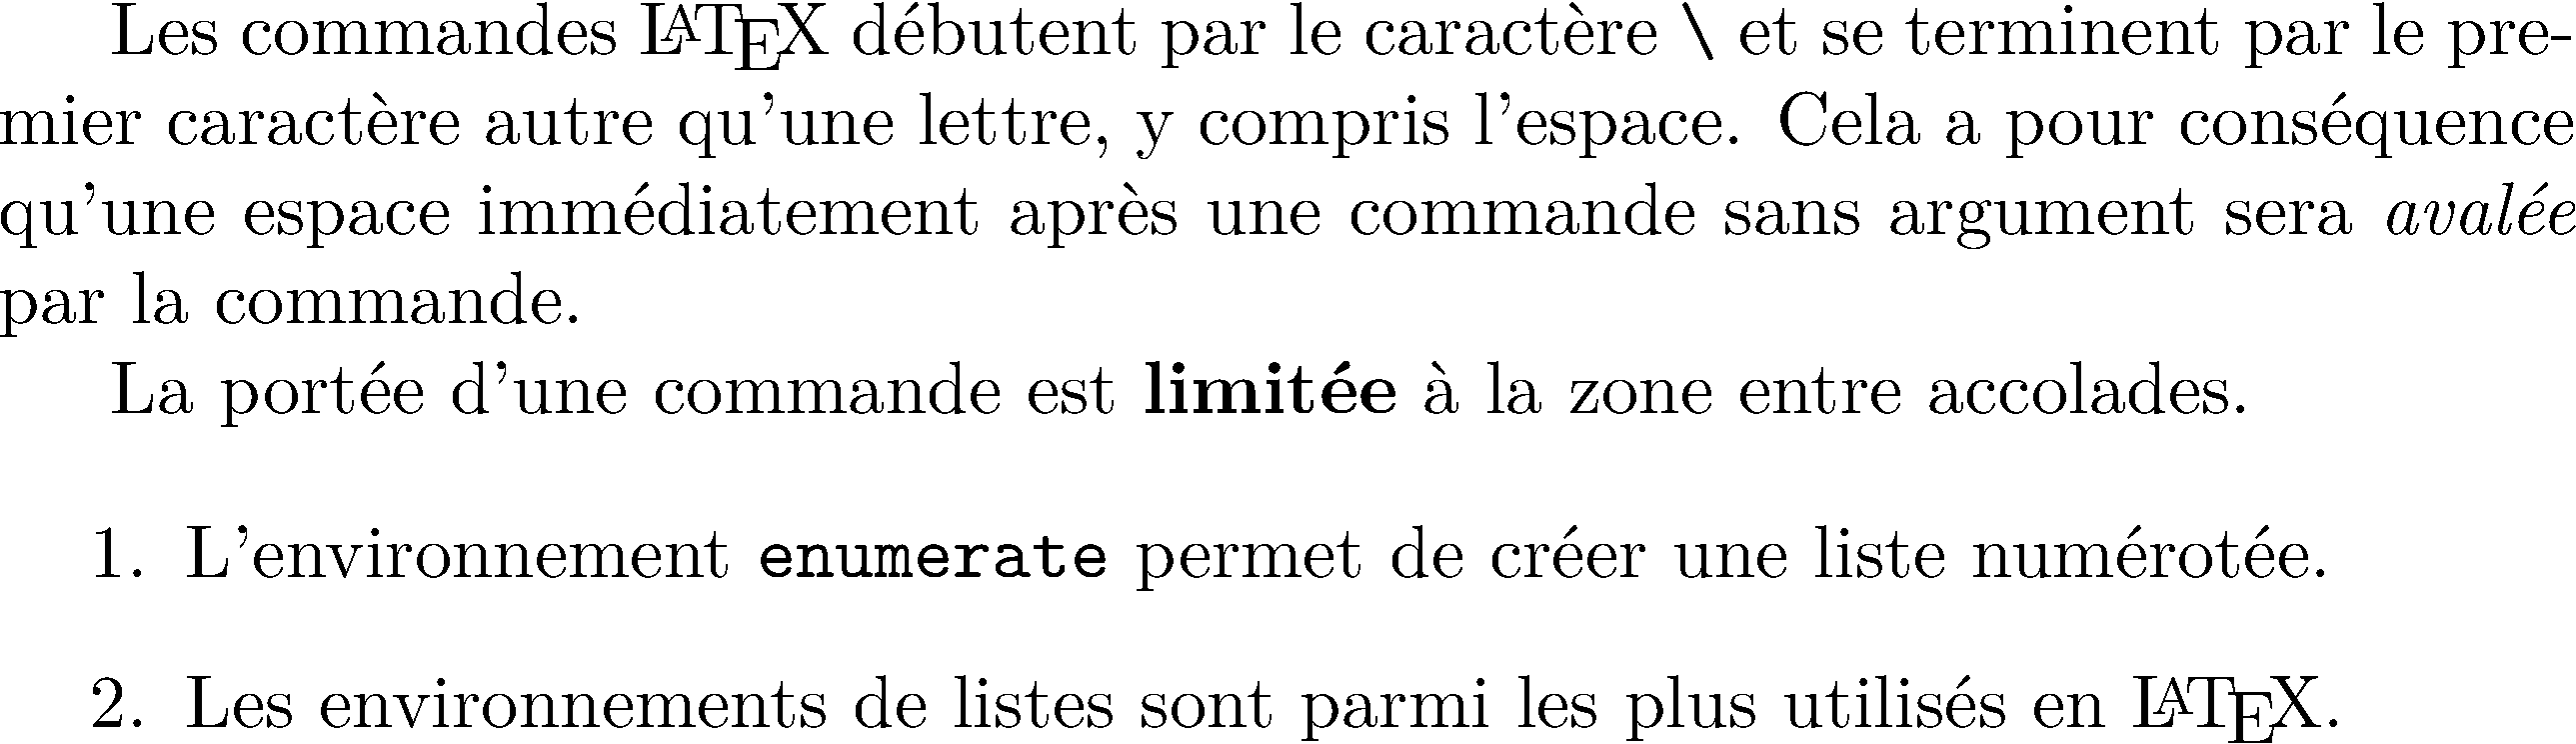
\includegraphics[width=0.95\linewidth]{exercice_commandes-output}
  \end{center}
\end{exercice}

\begin{exercice}[nosol]
  \begin{enumerate}
  \item Compiler tel que fourni le fichier
    \fichier{exercice\_classe+paquetages.tex}.
  \item Changer la police de caractère du document pour 11~points,
    puis 12~points. Changer la classe du document pour \class{memoir}.
    Observer l'effet sur les marges et sur la coupure automatique des
    mots.
  \item Charger le paquetage \pkg{icomma} et observer l'effet sur la
    formule mathématique.
  \item Charger le paquetage \pkg{numprint} avec l'option
    \verb=autolanguage= (\emph{après} le paquetage \pkg{babel}). Dans
    le code source de la formule mathématique, changer
\begin{lstlisting}
10 000
\end{lstlisting}
    pour
\begin{lstlisting}
\nombre{10000}
\end{lstlisting}
    et observer le résultat.
  \end{enumerate}
\end{exercice}

%%% Local Variables:
%%% mode: latex
%%% TeX-engine: xetex
%%% TeX-master: "formation-latex-ul"
%%% coding: utf-8
%%% End:
